\chapter{Security Measures}\label{chapter:security_measures}

This section describes all security features of the \gnb{} application, while discussing the details of each measure, how the feature was Implemented and what security threat(s) this measure protects from.
\clearpage
\subsection{Proper server configuration}
\securityMeasure{%
	The web server environment was configured appropriately, in order to protect the server and the web application itself from malicious attackers.
}{%
	The apache2 server was manually configured to disable all directory listing, as well as to prevent all access to files contained in directories that should not be directly accessible via browser (such as the contents of the \texttt{/project/lib} folder). Only PHP, Javascript and CSS files residing in specific folders of the web application can be referenced directly via browser. In this particular case, this was handled with a black-list.
}{%
	A valid server configuration prevents information leakage, usually caused by enabled directory listing or direct access to sensitive information (refer to OTG-CONFIG-001).
}

\clearpage
\subsection{HTTPS with HSTS}
\securityMeasure{%
	The site is only reachable over HTTPS and employs HSTS (HTTP Strict
	Transport Security) to protect against a downgrade of future connection
	attempts to HTTP.
}{%
	The apache2 server was configured in a way that only allows connections via
	HTTPS and always appends the \texttt{Strict-Transport-Security} header to
	replys to enable HSTS in the clients browser.
}{%
	\begin{itemize}
		\item Capturing of the communication between the client and the server
			by an third party.
		\item Modification of the communication between the client and the
			server by a man-in-the-middle attacker.
		\item Downgrade of a new connection to the server to HTTP by a
			man-in-the-middle attacker (after an initial connection to the correct
			site)
	\end{itemize}
}


\clearpage
\subsection{SSL secure ciphers}\label{sec:ssl_ciphers}
\securityMeasure{%
	The SSL ciphers offered by the webserver for HTTPS connections are
	configured to confirm the latest standards.
}{%
	The apache2 server was configured to only offer ciphers that are
	known secure.
	As visible in \autoref{figure:ciphers1} and \autoref{figure:ciphers2},
	current SSL testing tools give the site a perfect score.
}{%
	Save against SSL vulnerabilities. E.g.\ Heartbleed, POODLE, FREAK.
	Prevents eavesdropping and man-in-the-middle attacks caused by weak ciphers.
}
\begin{figure}[h!tbp]
	\centering
	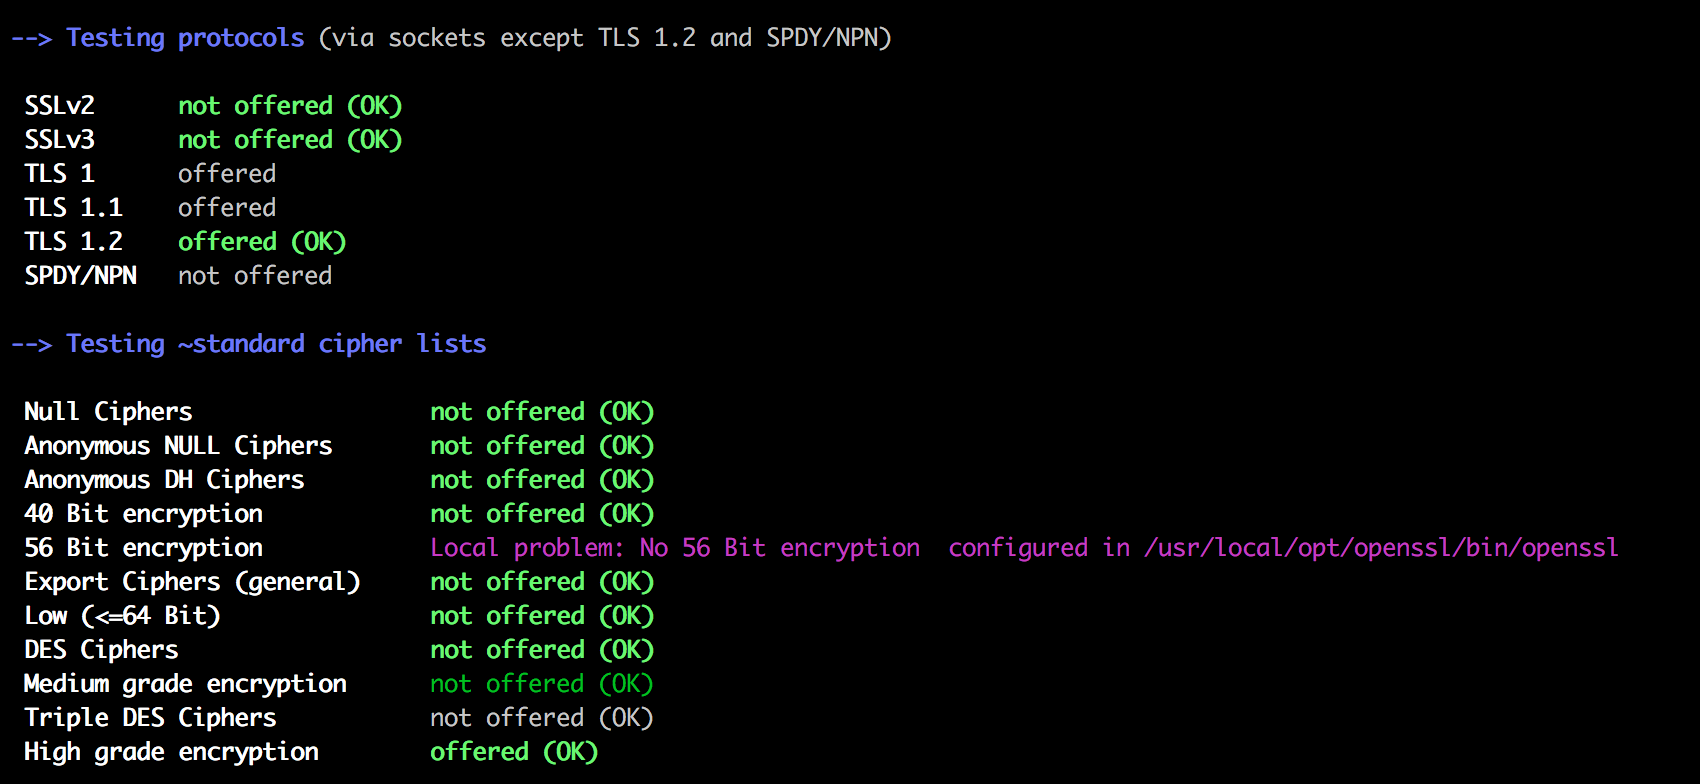
\includegraphics[width=\textwidth]{figures/ciphers1}
	\caption{Available SSL Ciphers}
	\label{figure:ciphers1}
\end{figure}
\begin{figure}[h!tbp]
	\centering
	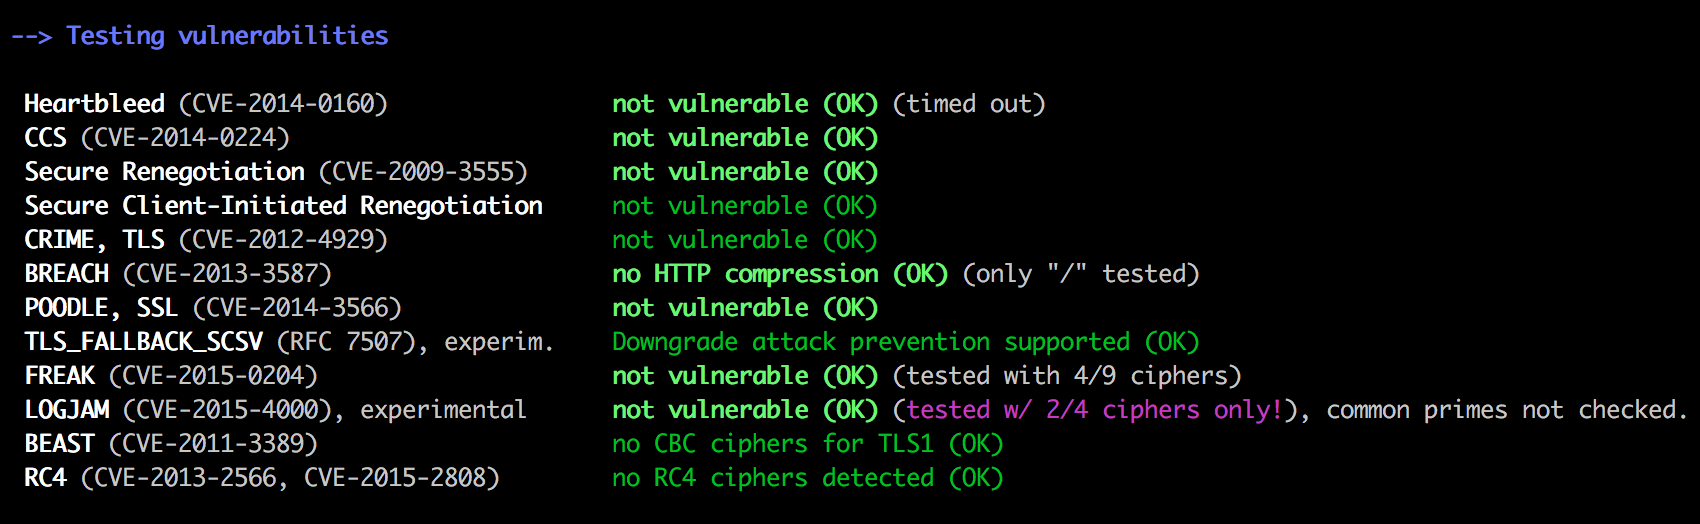
\includegraphics[width=\textwidth]{figures/ciphers2}
	\caption{No known SSL Vulnerabilities}
	\label{figure:ciphers2}
\end{figure}


\clearpage
\subsection{CSRF tokens}
\securityMeasure{
	The application automatically creates anti-CSRF cryptographic nonces (tokens) on all pages with forms that could be exploited to perform operations using the profile of a user. These tokens are validated once the form is submitted by the user, ensuring that the application can't be forced to perform actions via cross-site requests.
}{
	This feature was implemented manually, by creating a 256-bit random token (obtained via the PHP builtin \texttt{openssl\_random\_pseudo\_bytes} function) and encoding it base64. This token is then saved as a session variable and sent to the user as a hidden field inside a form, as can be seen in the figure below. Once the form is submitted by the user, the the token contained inside the form is compared against the one already existing on the server.
}{
	This particular security feature protects against XSRF attacks, as described in OTG-SESS-005.
}
\begin{figure}[h!tbp]
	\centering
	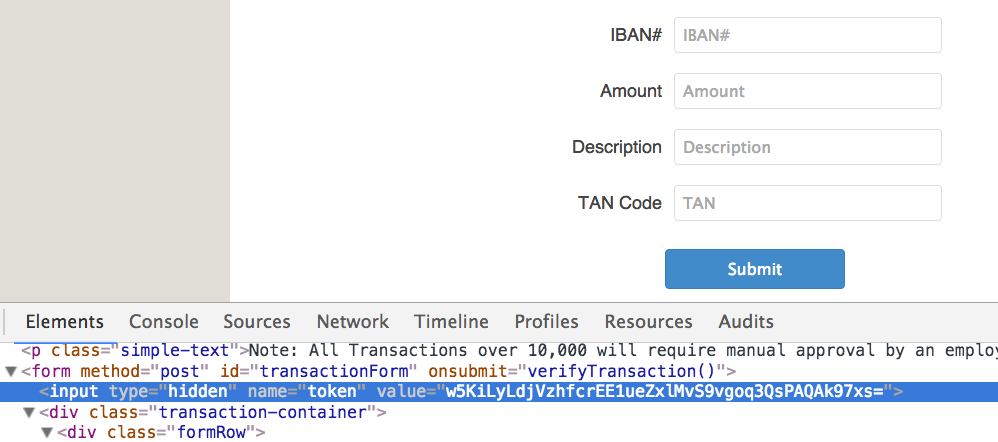
\includegraphics[width=\textwidth]{figures/csrf_token}
	\caption{CSRF token generated in the transaction page}
	\label{figure:csrf}
\end{figure}


\clearpage
\subsection{Password strength}
%Sample table
\securityMeasure{%
	We enforce strong passwords by forcing the users to respect the following criteria:
	\begin{itemize}
		\item length between 8 and 20 characters;
		\item at least 1 numeric character (0-9);
		\item at least 1 upper/lower case letter (a-zA-Z);
		\item any special character inside the password is allowed.
	\end{itemize}
	Any password not matching these criteria is rejected by the server.
}{
	The password enforcing mechanism was manually implemented both on client side (see \texttt{project/js/registration.js}) and on server side (see \texttt{project/registration/registration\_request.php}). The user is compelled to follow the mentioned criteria when choosing a password during registration. This also holds true when resetting a password later on.
}{
	Strong password prevent attackers from guessing them, as described in OTG-AUTHN-007.
}


\clearpage
\subsection{Secure passwords}
\securityMeasure{%
	User passwords are stored inside the database after a successful registration. Passwords are never stored in plaintext, but are hashed using a random salt, unique for every user, together with an additional static salt, known only to the backend server. 	
}{
	The algorithm used for hashing these values together is the SHA-512. A salt is generated for every user via the builtin PHP \texttt{openssl\_random\_pseudo\_bytes} function. The salt and the hashed password are both stored on the database (see \autoref{section:db}). No additional libraries were used to implement this feature.
}{
	Secure passwords protect the users in case the database is compromised in any way. An attacker is not able to determine which users are using the same password and cannot retrieve the original password, starting from the hashed one.
}


\clearpage
\subsection{Password reset with two-factor authentication}
\securityMeasure{%
	The user has the possibility to reset his password in case he does not remember it. A password reset requires the users mail address and access to the used mail account. Additionally the user has to enter his PIN to complete the process of resetting his password. This prevents attackers that already have access to the users mail address from resetting the password.
}{
	This has been implemented using the columns \texttt{pw\_reset\_hash}, \texttt{pw\_reset\_hash\_timestamp} and \texttt{pin} in the table \texttt{user}. When a password reset is requested a mail is sent to the user with a randomly generated token which is also stored in the database with the current timestamp. The user then has to use this token before it is invalidated by clicking on the link in the email, and providing a new password and the current PIN in the form.
}{
	This security feature protects users from attackers that already have access to their mail account, physical access to their device(s) or started the password reset process through social engineering.
}


\clearpage
\subsection{Lockout mechanism after failed password entries}
\securityMeasure{%
	In order to use our website users are required to log in. For a successful login the right username (which is the users mail address) and the correct password are required. To prevent brute force attacks given an already known mail address a lockout mechanism has been implemented. This mechanism blocks the user account if the wrong password has been entered 5 times in a row. The user has to be unblocked by an employee afterwards.

The same functionality was implemented to prevent brute force attacks on TANs for transactions.
}{
	This feature was implemented by adding the table \texttt{failed\_attempts} to the database (see \autoref{section:db}). This table stores all failed attempts (e.g. login or an invalid TAN) with the timestamp of the attempt and the ID of the user that executed the action. Every time an invalid password or TAN is observed a failed attempt is added the database and the sum of all failed attempts is checked. Once a valid password or TAN is entered all failed attempts are reset.
}{
	This feature protects against Application Mis-Use (OTG-BUSLOGIC-007) and brute force attacks on the login functionality (OTG-AUTHN-003).
}


\clearpage
\subsection{Automatic logout after inactivity}
\securityMeasure{%
	The application automatically logs out users who have been inactive for 30
	minutes.
}{%
	This was implemented on two different levels. The
	\texttt{session.gc\_maxlifetime} setting in the php configuration allows
	sessions to be removed after 1440 seconds. Additionally the user is logged
	out by a check in the php code if it latest activity lies more than 30
	minutes in the past.
}{%
	Prevents stealing of the user session from the clients computer after the
	timeout.
}


\clearpage
\subsection{CAPTCHAs}
\securityMeasure{%
	During the registration process users are required to enter a CAPTCHA code in order to prevent malicious attackers from automating registrations. This CAPTCHA is entirely random and requires the user to read an image and input the alphanumeric code manually.
}{
	For the creation of the CAPTCHA we resort to the \texttt{secureimage} library (see \ref{chapter:application_architecture} for further info).
}{
	This security feature protects the application from attackers who try to automate registrations (see OTG-IDENT-002), which could lead to a database saturation or even to a DOS.
}


\clearpage
\subsection{Resource Mapper}
\securityMeasure{%
	When including any resource, be it PHP files, images or else, the application exploits a key-value store, in which all resources are kept. Each resource is defined by a logical name (the key), which can be used to query the resource mapper to obtain an absolute path to a specific resource (the value).
}{
	This feature was implemented via the \texttt{/project/resource\_mappings.php} file, in which all key-value pairs to identify resources are stored. Whenever a PHP file needs to include another resource, this resource is looked up using the API offered by the resource mapper. If a mapping to the queried logical name was found, the resource is then returned and included. More details can be found in \autoref{subsection:resmapper}.
}{
	By avoiding to directly include files specified by request parameters (or even user input), this feature protects the web application against file inclusion attacks (see OTG-AUTHZ-001).
}

\clearpage
\subsection{Balance calculated in database (Realtime concurrent transactions)}
\securityMeasure{%
	As described in \autoref{section:db} the balance for each given account is always calculated in realtime in the database. The \texttt{VIEW} \texttt{account\_overview} uses all existing transactions and determines its value for the given account using the transaction status, the destination account and source account. This not only ensures an always consistent database because it is not possible to remove the balance for one account and "forget" to update the balance for the other account, but also enables realtime concurrent transactions, because no locking is necessary when new transactions are added.
}{
	This feature was implemented using the SQL-\texttt{VIEW} \texttt{account\_overview} which combines the tables \texttt{account} and \texttt{transaction} to calculate the current balance for a  given account. The implementation of this \texttt{VIEW} is shown in \autoref{figure:accountoverviewfigure} and explained in \autoref{section:db}.
}{
	This security feature protects against flaws in the business logic data validation (OTG-BUSLOGIC-001) e.g. if actions are not completed successfully without taking necessary rollback steps. This also prevents exploiting a possible Circumvention of Work Flow (OTG-BUSLOGIC-006) as one transaction is an atomic operation. Summed up this feature ensures that the database is always consistent and no money can get lost due to incompletely handled transactions.
}


\clearpage
\subsection{Password protected PDFs for TAN lists}
\securityMeasure{%
	The TAN list sent out to new users upon approval is encrypted with a
	password which gets sent to the user over a separate channel.
}{
	We encrypt the TAN list PDF with a password derived from the user pin. The
	user gets this password displayed in the webinterface when he successfully
	logs in.
}{
	Interception of the TAN list as it's sent over an unencrypted channel
	(email).
}


\clearpage
\subsection{Time-based TANs generated via SCS}
\securityMeasure{%
	Each TAN, generated using the SmartCard Simulator, is unique and provides an intrinsec degree of randmness, as a timestamp is used for the creation of the TAN. Since the server stores on the database the timestamp of the last used TAN, it is not possible to reuse old TANs.
}{
	This mechanism was implemented in the SCS Java application (refer to \autoref{section:scs}), as well as on the backend server, where TANs are validated and the timestamp is saved on the database (see the \texttt{verify\_transaction.php} file).
}{
	This feature prevents malicious attackers from attempting replay attacks in case they managed to obtain a TAN generated by a user. This could only occur if an attacker had access to the system of the victim, but even in that case, a TAN can never be reused.
}


\clearpage
\subsection{Secure cookies}
\securityMeasure{%
	A secure cookie is a cookie that contains a special \lq{} HttpOnly \rq{} flag included in the http cookie header that ensures cookies will only be used when transmitting HTTP (or HTTPS) requests.
	Combined the Secure setting and HttpOnly flag help to introduce a more robust cookie that is less prone to attacks. 
}{
	This is done by setting the \textbf{session.cookie\_secure} and \textbf{session.cookie\_httponly} in the \textbf{php.ini} to \textbf{1}
}{
	This allows the browser to restrict access to secure cookie data from scripts within the web browser. This limits the potential damage many cross site script attacks can cause -specifically-, the attacks that target cookie data.
}

\clearpage
\subsection{Input sanitization}

\securityMeasure{%
	Input sanitization is processing user input by removing  any malicious code that the user may have inserted in the input fields and converting any special characters to HTML friendly representations, before passing it on to other parts of the application such as SQL, HTML or PHP.
}{
	Functions were created to sanitize inputs based on the type of the input field, the functions exist in the  \textbf{project/genericfunctions.php} file.
}{
	This prevents against XSS, Command Injection and SQL injections.
}

\clearpage
\subsection{Prepared statements}
\securityMeasure{%
	Prepared statements are SQL statements that are pre-written and only missing one or more variables, the DB then parses, compiles and performs query optimization on the SQL template and stores the result without execution, The application at a later time binds the values to the parameters and executes the statement.
}{
	This was implemented using the PHP Data Objects (PDO) Extension. 
}{
	Prepared statements are very useful against SQL injections, because parameter values, which are transmitted later using a different protocol, need not be correctly escaped. If the original statement template is not derived from external input, SQL injection cannot occur.
}

\clearpage
\subsection{Clickjacking prevention}
\securityMeasure{%
	This prevents the Clickjacking attack which is the malicious practice of manipulating a website user\textsc{\char13}s activity by concealing hyperlinks beneath legitimate clickable content, thereby causing the user to perform actions of which they are unaware.
}{
	This was accomplished by denying X-Frame-Options, which was done by adding \newline
	\textbf{Header always set X-Frame-Options DENY} \newline
	in the \textbf{httpd.conf}.
}{
	Clickjacking.
}
